\section{Teaching Assistant}

\subsection{Do I have to be a TA?}
\begin{itemize}
    \item If you are a full scholarship PhD student (tuition waiver + stipend), according to the Financial Offer from the school, you have TA obligations every semester (in other words, the scholarship is in exchange for TA work; you must work if you receive the money). After working as a TA, you will not receive additional wages. For full scholarship PhD students enrolled in 2020 and later, they must complete 900 hours of TA work over three years to graduate. For those enrolled in 2023 and later, they must complete 300-500 hours of TA or RA work each academic year to graduate.
    \item If you are a half-scholarship PhD student (tuition waiver only) or a self-funded student enrolled in 2020 and later, you have no obligation to work as a TA. After working as a TA, the school will pay you according to the hours worked, and the TA experience can be added to your resume, which might be beneficial depending on your future career plans.
\end{itemize}

For full scholarship students, the mandatory 300 hours of TA work per academic year equates to approximately 7.5 hours of duty per week over 40 teaching weeks, roughly equivalent to one day per week. You might wonder if this is strictly enforced. In practice, enforcement varies significantly between colleges. Some colleges have established a digital system to track your hours, requiring you to meet the quota, while others are more lenient. For specific enforcement details, please consult senior students in your program.

\begin{flushright}
    (2022年10月21日 by \Wu)

    (major update: December 30, 2022 by Yue Zhou: Updated TA hours according to the latest official handbook)

    (update: January 15, 2024 by \Wu : Updated TA hours according to the latest official handbook)

    (Translated by GPT)
\end{flushright}

\subsection{How to Become a TA}

Around the first week of each semester, the college will recruit TAs, usually through the School Academic Administrator.
\begin{itemize}
    \item Half-scholarship and self-funded PhD students have more freedom and can contact the course instructors directly.
    \item Full scholarship PhD students have two scenarios: a) contacting course instructors directly, or b) being assigned by the college via email.
\end{itemize}

If you are eager to participate or want to secure a spot in a particular course or with a specific instructor, contact the administrator and the relevant course instructor as early as possible.

\begin{flushright}
    (December 30, 2022 by Yue Zhou) \\
    (Translated by GPT)
\end{flushright}

\subsection{Types of TA Work and How to Do Them}

TA duties include but are not limited to:
\begin{enumerate}
    \item Grading assignments and exams
    \item Conducting tutorials (mostly in business courses) and labs
    \item Calculating and recording course grades
    \item Performing auxiliary tasks (e.g., setting up Learning Mall)
    \item Proctoring midterm and final exams
\end{enumerate}

The Graduate School organizes TA training sessions, which are announced via emails titled \textit{Teaching Assistant (TA) Training Programme} and can also be found on your Learning Mall. These sessions are held every semester. If you have never attended any, it is recommended to attend at least once. Below are some core contents that the school’s training might not cover in detail:

\subsubsection{Grading Assignments}
If grading traditional paper-based assignments, generally ask the instructor how to proceed. For electronic assignments submitted through the Learning Mall (referred to as LMO), here is a tutorial:
\begin{enumerate}
    \item Log in to LMO and find the course you are assisting. If you cannot find it, email your school administrator or the course instructor to grant you access.
    \begin{figure}[H]
        \centering
        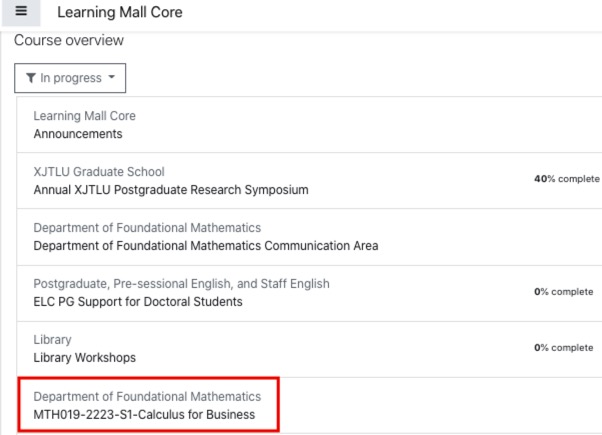
\includegraphics[width=0.4\columnwidth]{author-folder/Kai.Wu/LMO_course.jpg}
    \end{figure}

    \item 
    \begin{minipage}{0.3\textwidth}
        Enter the course, scroll down to find the submission area, or use Ctrl+F (Command+F on Mac) to search for “submission”.
    \end{minipage}
    \begin{minipage}{0.63\textwidth}
        \begin{figure}[H]
            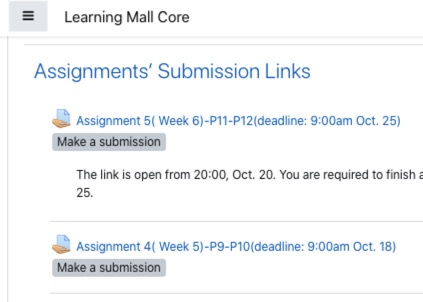
\includegraphics[width=0.95\columnwidth, right]{author-folder/Kai.Wu/LMO_submission_links.jpg}
        \end{figure}
    \end{minipage}

    \item For large required courses with many sections, first select the group you are assigned to grade. Next, if you want to start grading online immediately, click “Grade.” If you want to review or grade offline (e.g., download to an iPad), click “View all submissions.”
        \begin{figure}[H]
            \centering
            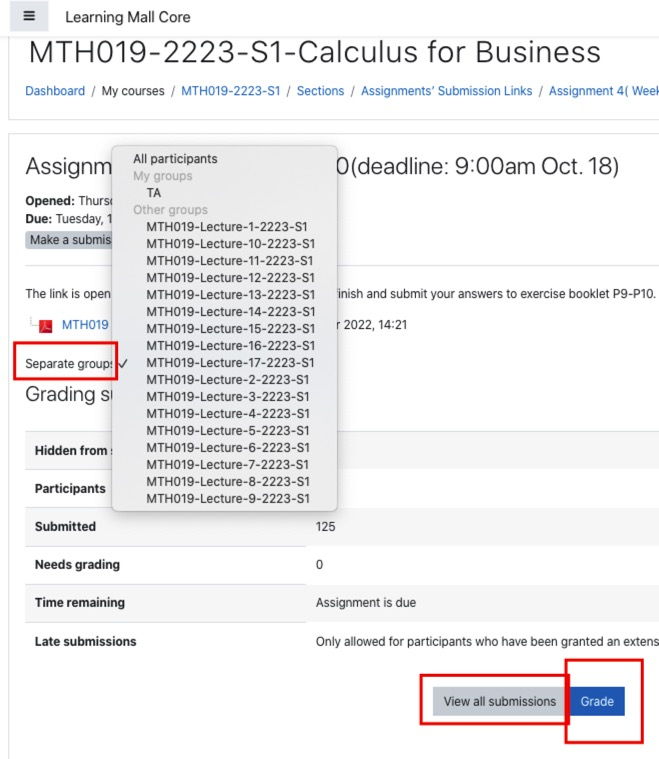
\includegraphics[width=0.5\columnwidth]{author-folder/Kai.Wu/LMO_inside_submission.jpg}
        \end{figure}
    \item The online grading system can be very slow and the PDF annotation tools are cumbersome, making online grading inefficient unless the instructor has provided a grading rubric (my advisor showed me once where you can select scores and reasons for each part of the assignment directly on the right side). Otherwise, online grading is not very useful. Below is a relatively efficient offline grading method I have figured out. After clicking “View all submissions,” select “Download grading worksheet” and “Download all submissions” from the “Grading action” menu.
        \begin{figure}[H]
            \centering
            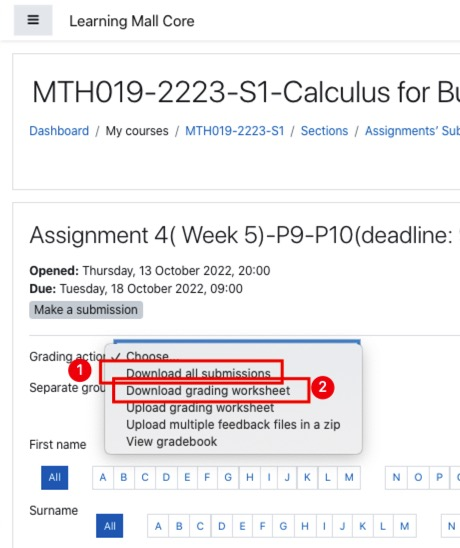
\includegraphics[width=0.5\columnwidth]{author-folder/Kai.Wu/LMO_download.jpg}
        \end{figure}
    \item You will receive a CSV file and a large ZIP file. Extract the ZIP to see all the student submissions named by student name and ID. You can then grade these files locally on your computer or tablet. If your instructor does not require the graded assignments to be returned as feedback files (ask your instructor), you can even print them out to grade. After grading, record the grades in the grading worksheet. The CSV can be opened with Excel, and you can save it as an XLSX file. The last column of the spreadsheet is “Feedback comments,” where you can write comments for students, such as “incorrect file format” or “please submit clearer images next time.”
        \begin{figure}[H]
            \centering
            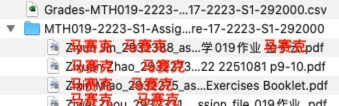
\includegraphics[width=0.5\columnwidth]{author-folder/Kai.Wu/LMO_Downloaded.jpg}
        \end{figure}
    \item After grading according to the instructor’s requirements, you can easily upload the grading worksheet and graded files (if required) back to LMO. From the “View all submissions” page, click “Upload grading worksheet” to upload the grading worksheet.
        \begin{figure}[H]
            \centering
            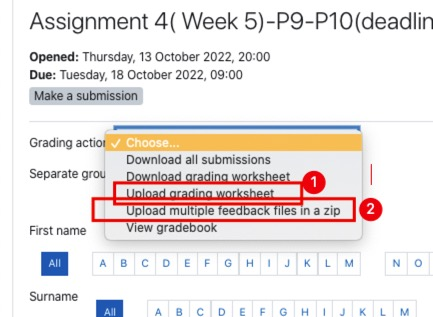
\includegraphics[width=0.5\columnwidth]{author-folder/Kai.Wu/LMO_upload.jpg}
        \end{figure}
    \item If you saved the worksheet as an XLSX file, save it as a UTF-8 CSV file before uploading. Check the “Allow this CSV to override existing grades” box. After clicking “Upload,” you will see a long webpage with each student’s grade and your feedback comments uploaded. 
        \begin{figure}[H]
            \centering
            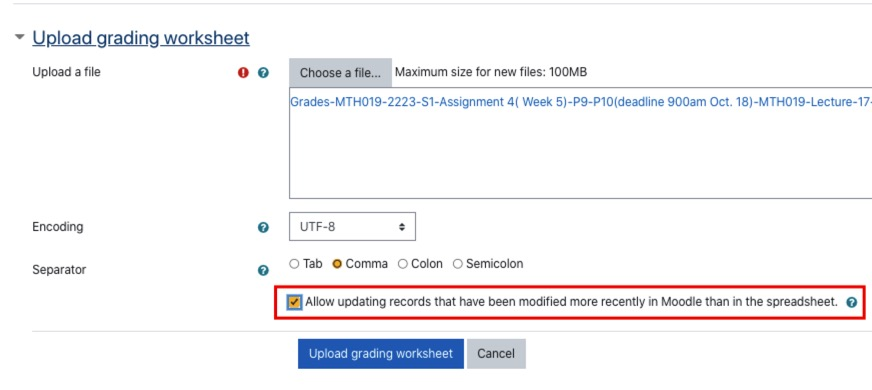
\includegraphics[width=0.8\columnwidth]{author-folder/Kai.Wu/LMO_upload_sheet.jpg}
        \end{figure}
    \item From the same page, click “Upload multiple feedback files in a ZIP” to upload the graded assignments. Zip the graded files, but if the total size exceeds 100MB, you will need to manually split them into multiple ZIP files smaller than 100MB (annoying, but LMO restricts uploads to 100MB). If you know Python, you can use my script \href{https://github.com/kaiwu-astro/xp_pgrs_unofficial_guide/tree/main/fileshare/zip_in_100M.py}{GitHub repo} or \href{https://gitee.com/kaiwu-astro/xp_pgrs_unofficial_guide/tree/main/fileshare}{Gitee repo} to automatically split the files into 100MB ZIPs. After uploading, you are done.
    \item Finally, email the instructor to report (1) common issues, such as frequently missed questions or common misunderstandings, (2) individual issues, such as students submitting the wrong files, suspected plagiarism, or similar assignments, and (3) any other issues you want to discuss with the instructor. The math department has a feedback form for this purpose. If there is no feedback form, you can email the instructor. (Generally, you don’t need to be too detailed unless you are passionate about this work, as it can be time-consuming.) 
        \begin{figure}[H]
            \centering
            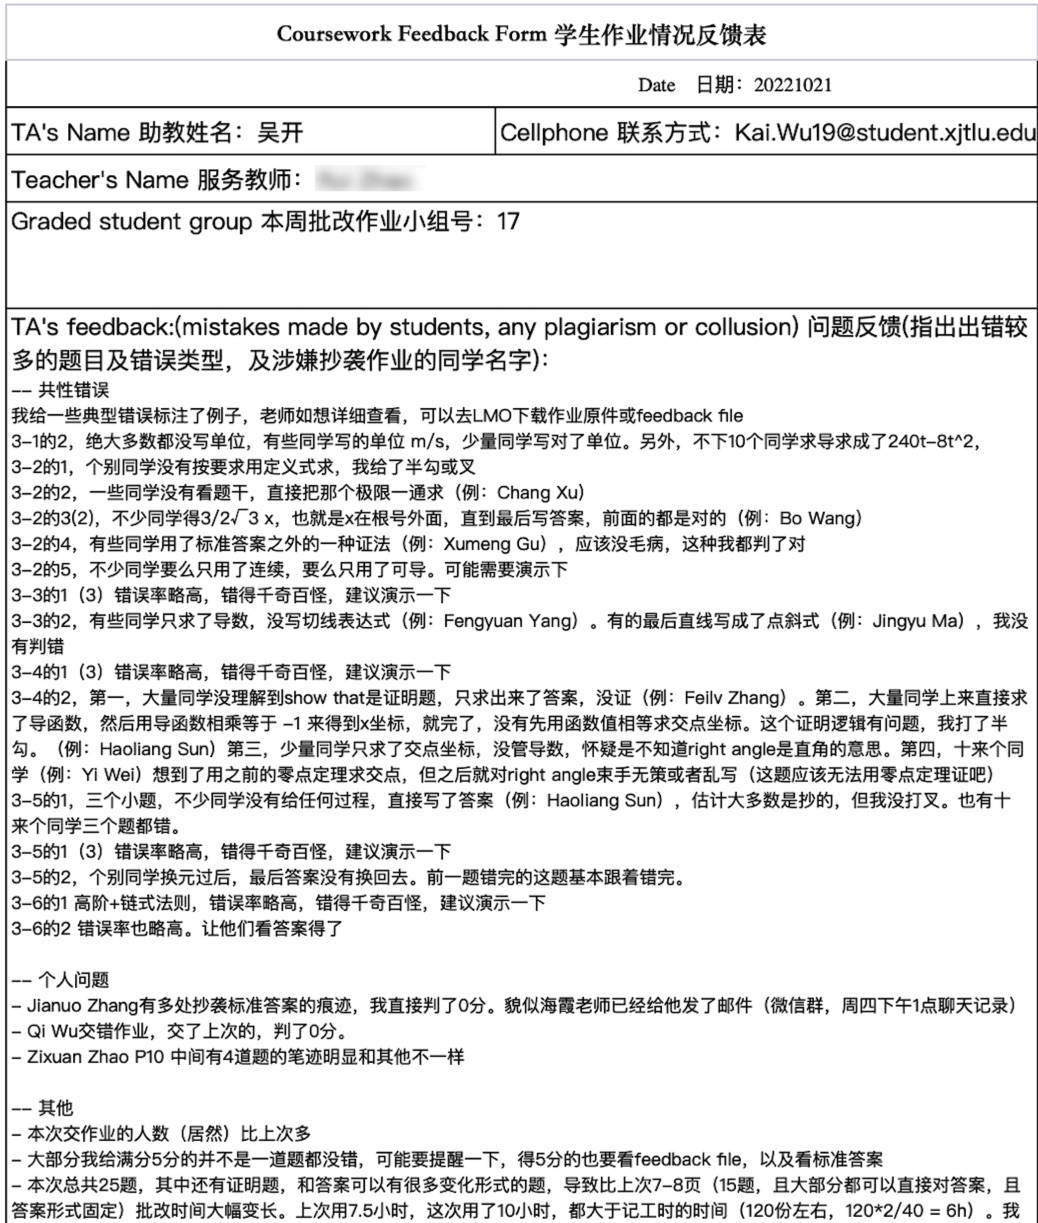
\includegraphics[width=0.5\columnwidth]{author-folder/Kai.Wu/LMO_feedback_to_teacher.jpg}
        \end{figure}
\end{enumerate}


\emptyline
Tips for Grading Assignments
\begin{enumerate}
    \item My tool combination is an iPad + Apple Pencil + PDF Expert app, which is much faster than grading online or offline on a computer. Additionally, purchasing a magnetic paper-like screen protector (about 20 yuan) and replacement pencil tips (about 10 yuan) can significantly improve the writing experience.
        \begin{figure}[H]
            \centering
            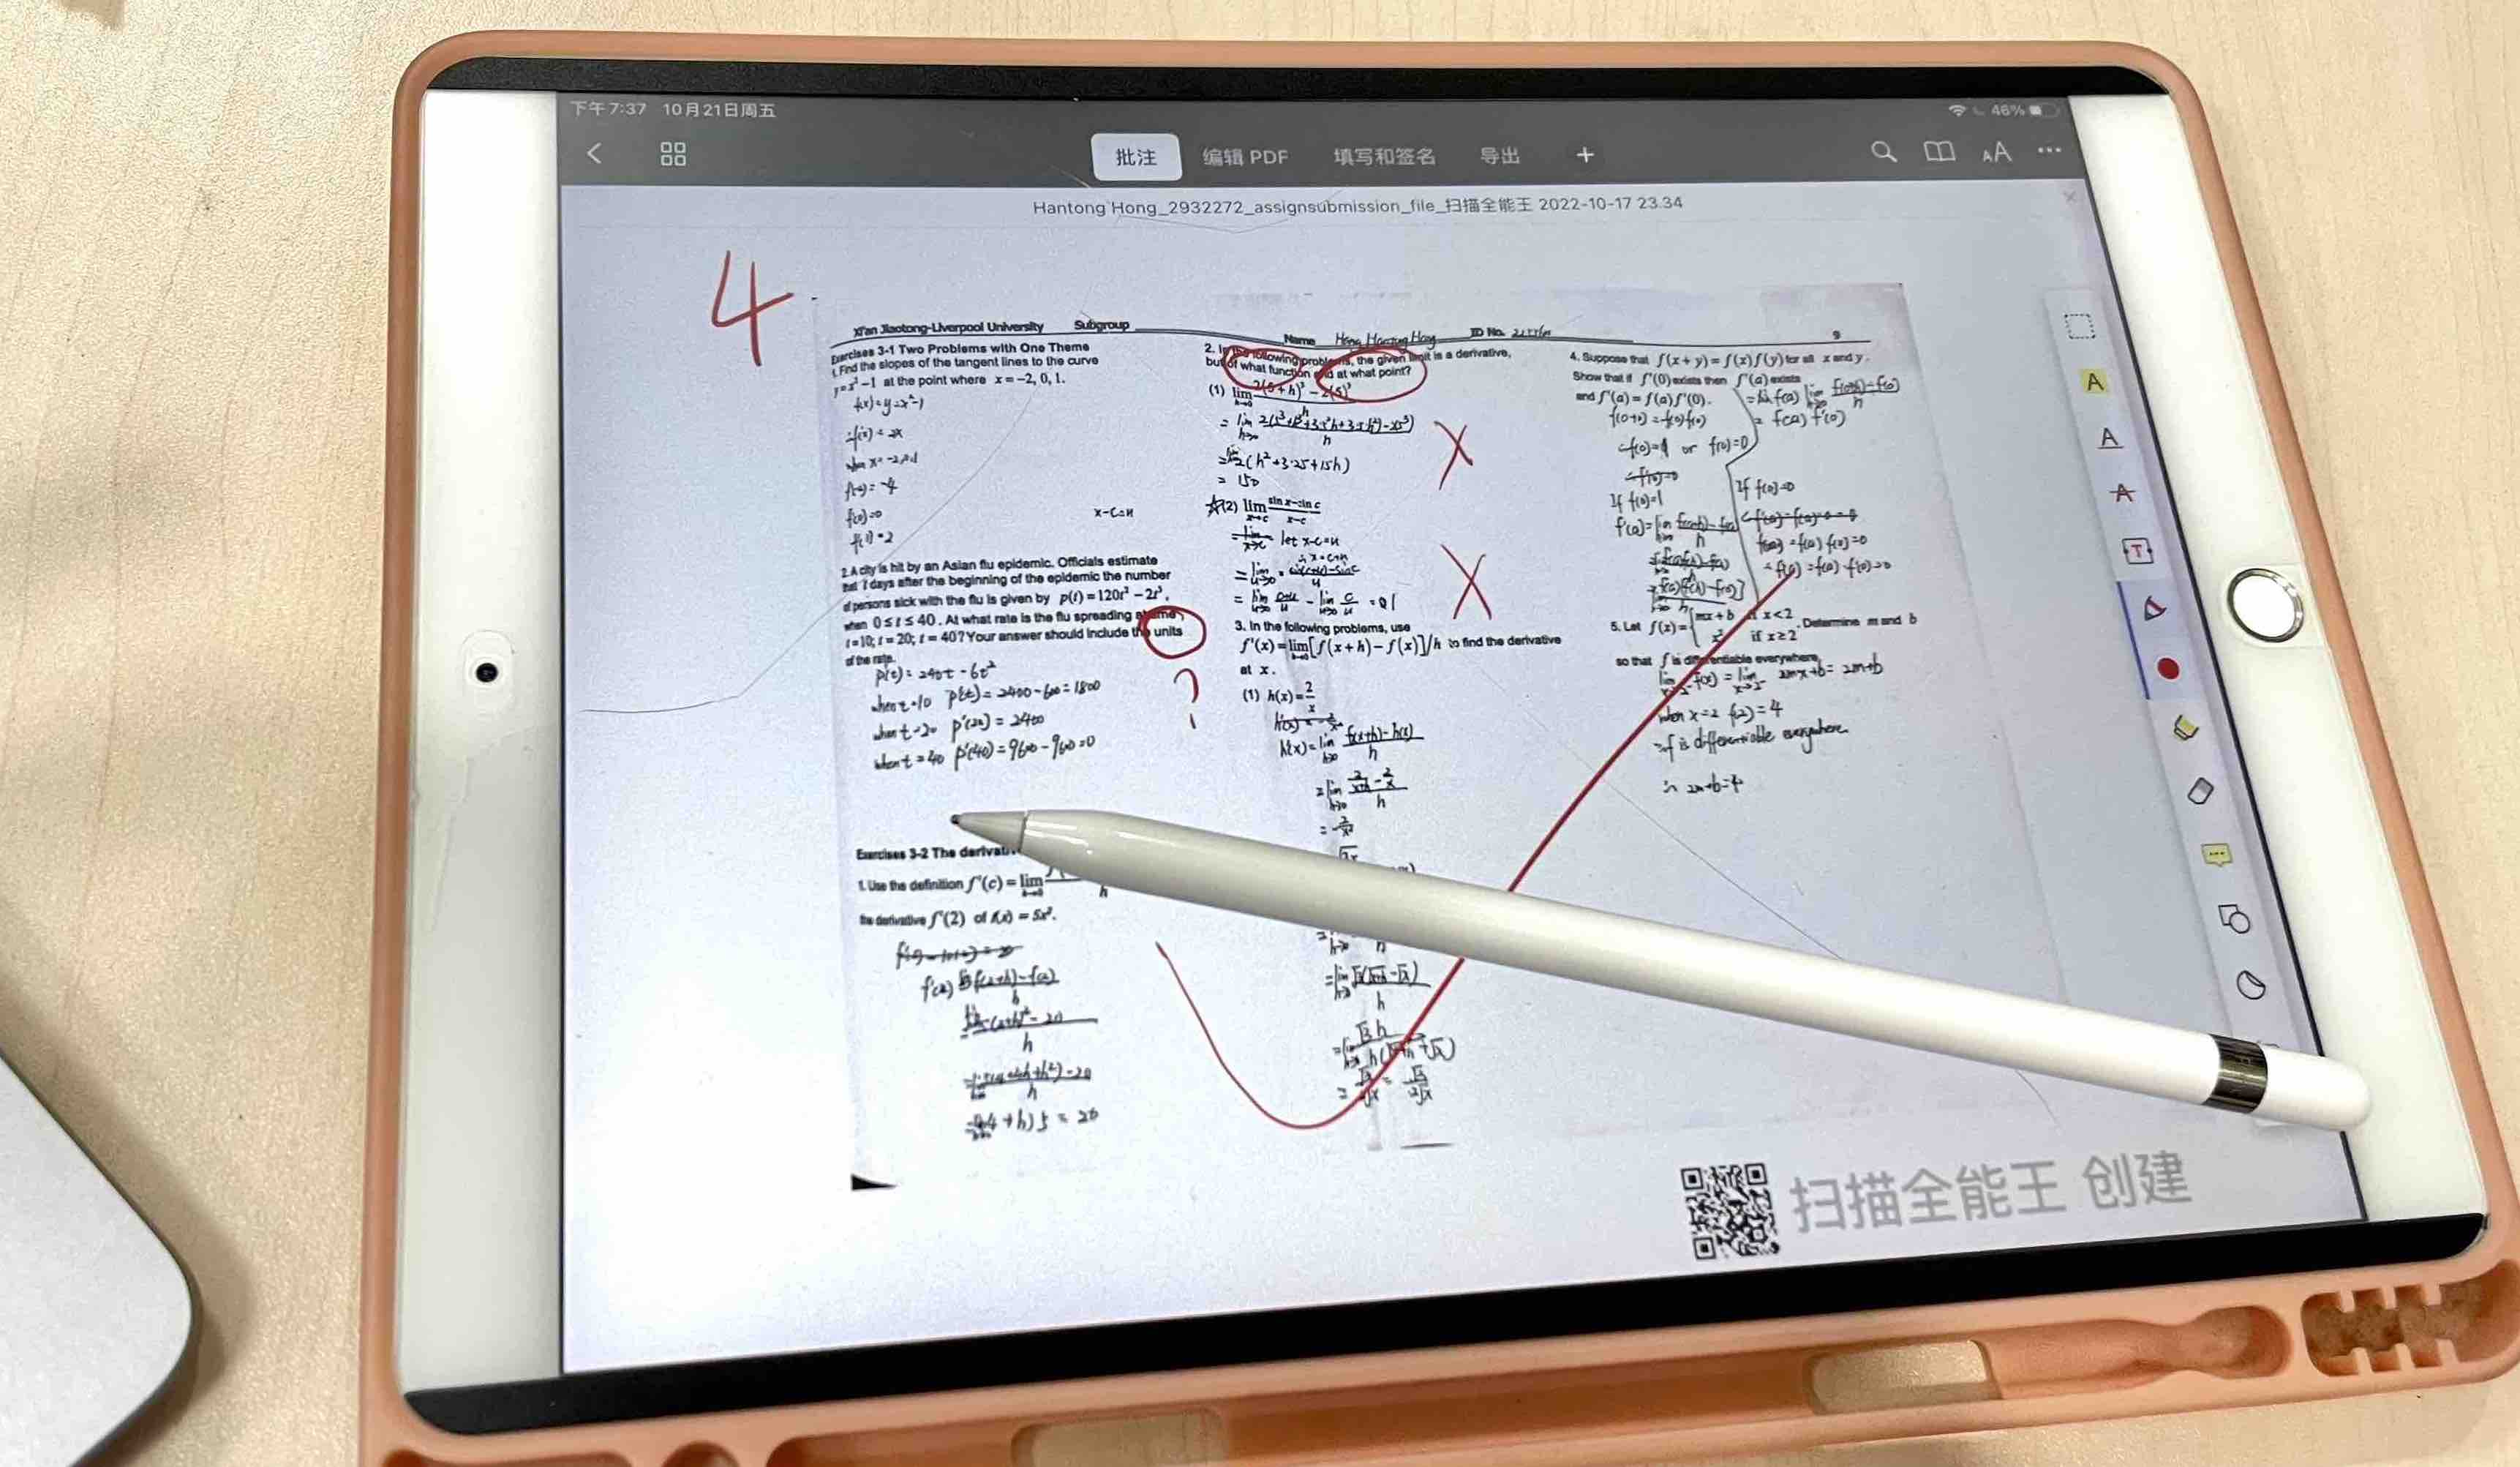
\includegraphics[width=0.5\columnwidth]{author-folder/Kai.Wu/marking_tools.jpg}
        \end{figure}
    \item Improve efficiency with an assembly line approach: When there are many questions, don’t grade all parts of one student’s assignment before moving to the next. Instead, grade all assignments’ part 1 (e.g., the first three questions), then go back and grade all part 2 (e.g., questions 4-6).
    \item Although opening and closing files takes time, this method helps you remember the answers and grading points, speeding up the process. Avoid looking at the answers for each assignment.
Similarly, don’t record grades one by one. My habit is to write the total score in large numbers in the top left corner. After grading all assignments, use the largest thumbnail view (Mac: View as Icons, press Command+Equal repeatedly; Windows: View as Extra Large Icons) to see the scores without opening the files. Sort by name in both Excel and the folder to quickly record the grades.
        \begin{figure}[H]
            \centering
            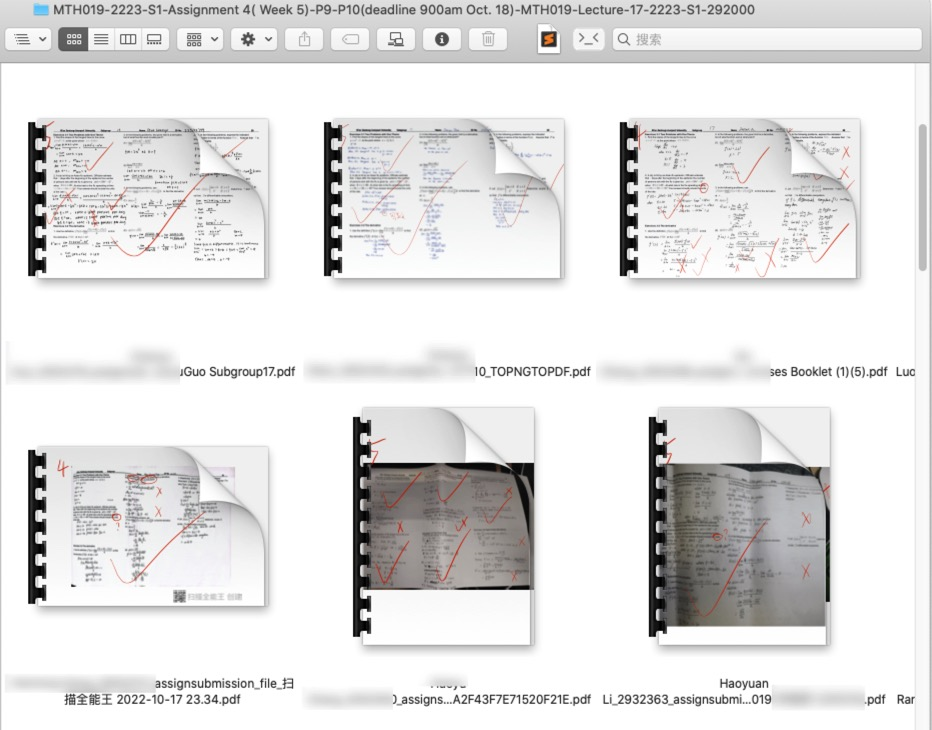
\includegraphics[width=0.7\columnwidth]{author-folder/Kai.Wu/tongchengji.jpg}
        \end{figure}
    \item Students may submit files with various issues, such as submitting Word or PPT instead of PDF, submitting PDFs with images in the wrong order or orientation, or writing on notebooks instead of using standard templates. TAs have the right to require students to follow specific formats and can warn students in the feedback comments. Remind the course instructor to emphasize this in class. If students continue to submit incorrect formats, you can deduct points according to your standards (e.g., first warning, second time deduct 20\%, third time deduct 50\%, fourth time deduct all).
    \item Sometimes, large files or files with many handwritten notes cause PDFs to open slowly or crash. For large files, ask students to compress the PDFs. For handwritten notes, there is no good solution. I wrote a Python script \href{https://github.com/kaiwu-astro/xp_pgrs_unofficial_guide/tree/main/fileshare/pdf_to_png_to_pdf.py}{[GitHub Link]}to convert PDFs to images and back to PDFs, making them open faster and reducing file size to under 5MB. Use it if needed, but it’s a bit complicated. I couldn’t find a better method.
    \item (Quietly) When unsure about the score, give a bit more. If you give too little, students will argue, wasting time. Giving a bit more saves your time.
    \item When recording grades, mistakes are inevitable, especially for new TAs. Consider double-checking everything. Writing the grade on the top left of the PDF helps, as students can see discrepancies between LMO and PDF grades and contact you.
    \item After grading, students may message you through LMO or email. Avoid replying directly to students, as mistakes can cause issues for the instructor. Forward all student messages to the instructor and let them reply unless they allow you to respond directly.
\end{enumerate}

\begin{flushright}
    (October 21, 2022 by \Wu) \\
    (Translated by GPT)
\end{flushright}

\subsubsection{Grading Exams}
For quizzes, midterms, and final exams, TAs may need to participate in grading. Before leaving for vacation at the end of the semester, confirm with the instructor to avoid missing grading responsibilities. If you need to leave early, discuss it with the instructor.

\subsubsection{Conducting Labs}
\begin{minipage}[t]{0.55\textwidth}
    For courses like university physics labs, TAs may need to conduct lab sessions. The typical process involves explaining the experiment principles, data recording and processing, and precautions on the lab whiteboard, followed by a hands-on demonstration. After the class, TAs need to grade lab reports.

    I find lab sessions very challenging because they involve real teaching in a university setting. You need to prepare lessons, organize your thoughts, and anticipate students' questions. The course instructor will train TAs in the lab, and you must understand the experiments thoroughly. Handling emergencies, such as students damaging equipment, requires immediate consultation with the instructor. Although lab sessions are few and the total work hours, including grading lab reports, are less than grading assignments for most other courses, they are very rewarding. If you want to challenge yourself, give it a try. If not, request a transfer to another course with the instructor and the school administrator early on.
    \begin{flushright}
        (October 22, 2022 by \Wu) \\
        (Translated by GPT)
    \end{flushright}
\end{minipage}
%
\begin{minipage}[t]{0.45\textwidth}
    \begin{figure}[H]
        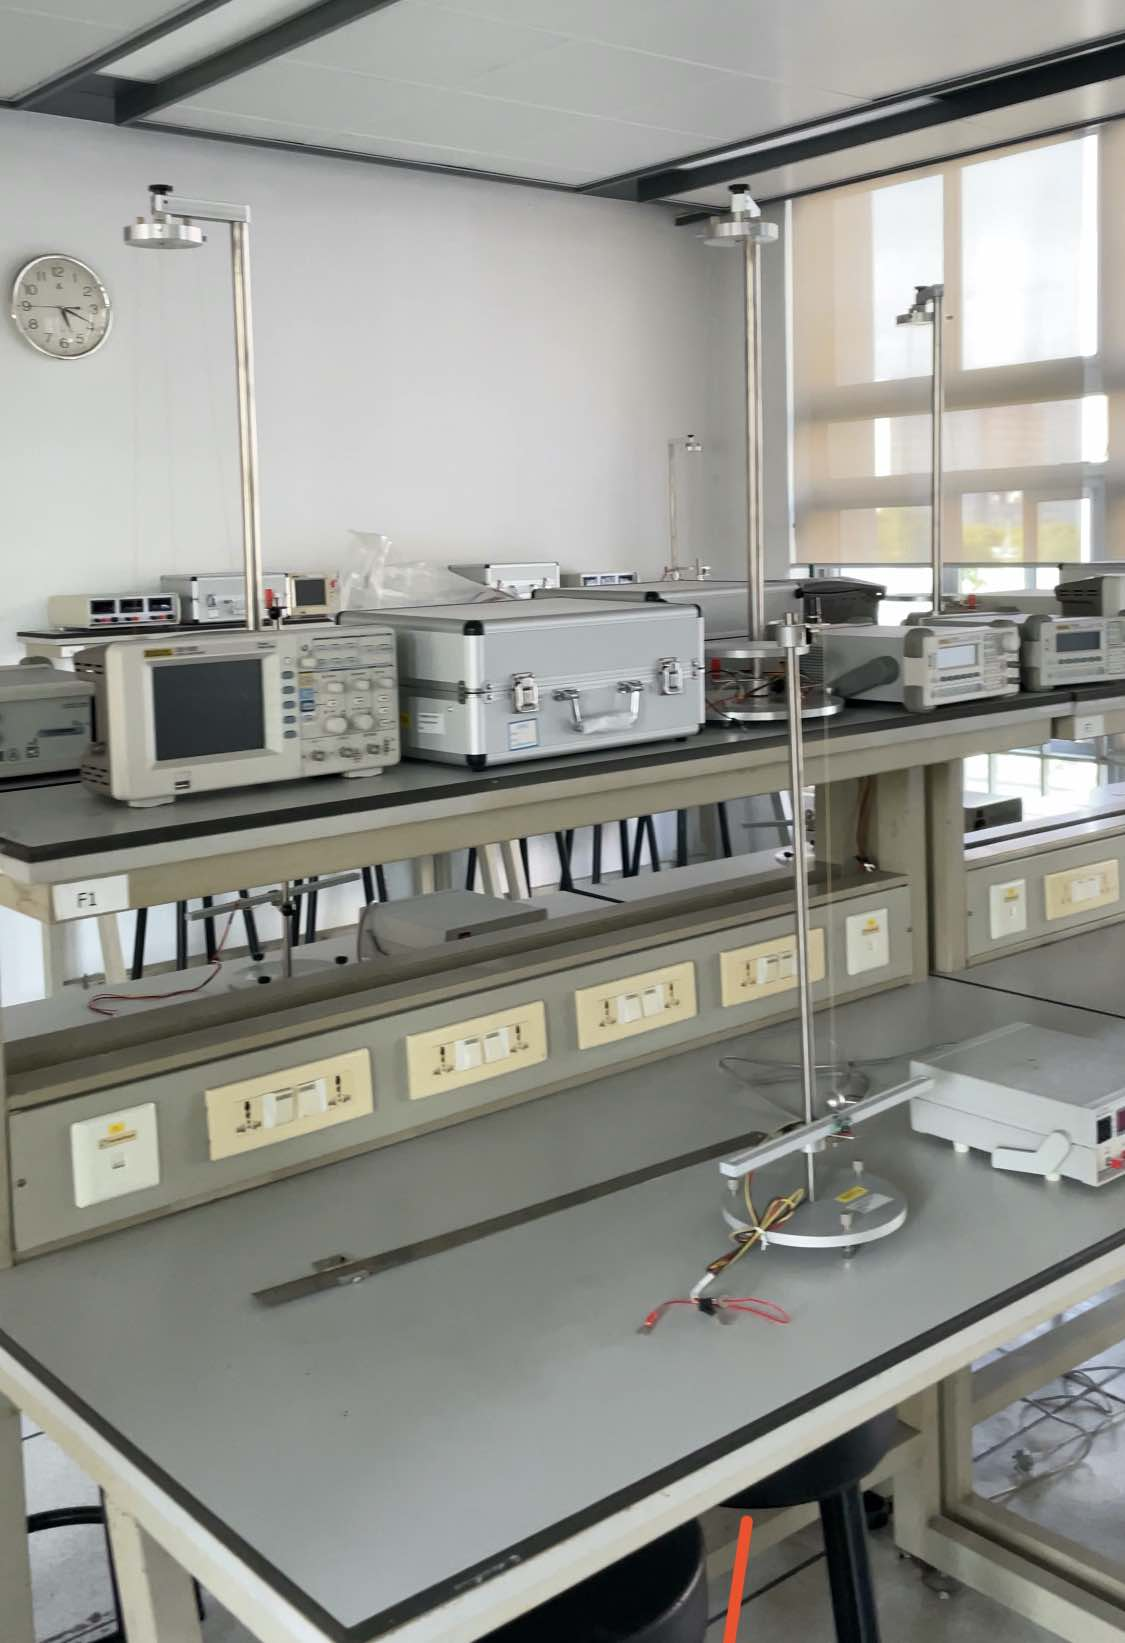
\includegraphics[width=0.95\columnwidth, right]{author-folder/Kai.Wu/lab.jpg}
    \end{figure}
\end{minipage}



\subsubsection{How to Conduct Tutorials}

\begin{enumerate}
    \item Prepare thoroughly before the class. When you stand on the podium, you are a teacher and must be responsible for everything you say and for the students. Copy the necessary materials to a USB drive before class, and log in to the classroom computer with your account to use it. You will also need to log in to systems like LMO and AMS. As the school computers are slow, arrive ten minutes early. Also, end the class ten minutes early to avoid complaints about going over time.
    \item Respond patiently to students’ emails and questions after class. Do not add students on WeChat lightly; ask them to contact you via email for any issues. Email is the official communication method in the school and protects the personal space and rights of teachers and TAs. There have been complaints about TAs not responding to students’ WeChat messages.
    \item Communicate with the module leader if you encounter difficult issues. Do not make decisions on your own; consult with the module leader. Share student feedback with co-teachers to improve the learning experience. Better student experiences lead to higher Module Questionnaire (MQ) scores. Good MQ scores can be included in your resume when job hunting.
\end{enumerate}

\begin{flushright}
    (October 30, 2022 by Yue Zhou) \\
    (Translated by GPT)
\end{flushright}

\subsection{TA Salary and Payment}
In 2022, the TA salary is 60 yuan per hour, paid monthly, with the salary for January work paid at the end of February.

\emptyline{}
Additionally, proctoring midterm and final exams is also considered TA work and will count towards scholarship students’ TA hours. Self-funded students are usually paid a higher hourly rate for proctoring. See the next section for more details on proctoring.

\begin{flushright}
    Translated by GPT
\end{flushright}